\section{Interaction Evaluation Strategies}
\label{sec:interaction-evaluation-strategies}
In order to determine which remote peers are providing valuable data and which peers are not, the local peer needs to be able to evaluate each interaction it had with the remote peer.
In general, there are two options for how to approach this, (i) by designing an evaluation that is protocol-aware (i.e. it understands the protocol and the data that the two peers shared ); or (ii) by having an evaluation function that does not need to understand the protocol and can be used for any type of data.

We choose to implement both approaches and they are described in the following sections. In order to evaluate which strategy is better in what scenarios, we designed and run many simulations - their results are described in the chapter \ref{ch:experiments}. 
We will use the notation from the table (\ref{table:interaction-eval})  when referring to peers and their interactions.

\begin{table}[h!]
\centering
\begin{tabular}{ c | m{20em} }
 $i$ & local peer \\
 \hline
 $j$ & remote peer \\
 \hline
 $T$ & target of network intelligence, domain or IP address \\
 \hline
 $k$ & evaluation window \\
 \hline
 $s^{k}_{i, j}$ & $i$'s satisfaction value with interaction with peer $j$ in window $k$\\
 \hline
 $S^{k}_{j, T}$ & score computed by the peer $j$ about target $T$ in window $k$ \\
 \hline
 $C^{k}_{j, T}$ & confidence, how much is the score correct \\
 \hline
 $S^{k}_{T}$ & aggregated score from all threat intelligence reports in window $w$ for target $T$ \\
 \hline
 $C^{k}_{T}$ & aggregated confidence
\end{tabular}
\caption{Interactions Symbols}
\label{table:interaction-eval}
\end{table}

\subsection{EvenTIEvaluation}
\label{subsec:same-eval-for-all-interactions}
This strategy does not need to understand the underlying data, its semantics, or its structure.
It is a naive approach when the trust model uses the same satisfaction value for all data it received. It does not check, if the data make sense and assigns all peers the same satisfaction value $s^{k}_{i, j}$.
The value itself is loaded from the configuration provided by the administrator. We denote it as $CSS$. 
The idea behind this algorithm is that when the peers are interacting for a long time or have more interactions, they're more trustworthy.

\begin{equation}
s^{k}_{i, j} = CSS
\end{equation}

This approach is for example used by the botnet \textbf{Sality} or by the \textbf{Dovecot} trust model. Fides implements it as an $EvenTIEvaluation$ strategy with configurable satisfaction value and the administrator can use this strategy if they see it as the most optimal.

The disadvantage of this approach is, that we do not penalize remote peers when they provide wrong data, because the evaluation method does not care nor understand the underlying data.
Because of that and in a case when the adversary gains the service trust of the model by following the protocol for a longer time, it may significantly influence the aggregated score as the adversary has higher trust than other remote peers. If this happens, there is no way to automatically downgrade the adversary's service trust.

\subsection{DistanceBasedTIEvaluation}
\label{subsec:distance-based-eval}
Because Fides is designed for sharing and aggregating threat intelligence, and understands the protocol that is being used, we can utilize this and penalize the peers that are providing the local peer with incorrect data.
The interaction evaluation is performed at the end of the threat intelligence sharing process, at that point, Fides already aggregated data and decided what is the aggregated network score and confidence. 
Thus, we can utilize aggregated values and use them as a baseline. Then we compare it against each remote peer's threat intelligence we received. This evaluation strategy is implemented in the Fides as a $DistanceBasedTIEvaluation$.

Suppose, that remote peer $j$ provided data about target $T$ to local peer $i$ in window $k$. Provided data consist of score and confidence ($S^{k}_{j, T}$, $C^{k}_{j, T}$). Where score,  $-1 \leq S^{k}_{j, T} \leq 1$, indicates if the target is malicious ($-1$) or begin ($1$). The confidence $0 \leq C^{k}_{j, T} \leq 1$ on the other hand indicates, how much is the peer sure about its assessment of $S^{k}_{j, T}$.

In order to evaluate interaction between the local peer $i$ and remote peer $j$ we need to compute satisfaction value $s^{k}_{i, j}$. 
It holds that  $0 \leq s^{k}_{i, j} \leq 1$ where $1$ means peer $i$ was satisfied with the interaction.

\begin{equation}
s^{k}_{i, j} = \left(1 - \frac{|{S}^{k}_{T} - S^{k}_{j, T}|}{2} \cdot C^{k}_{j, T}\right) \cdot C^{k}_{T}
\end{equation}

Where $S^{k}_{T}$ is the final score aggregated across the reports from the peers, $C^{k}_{T}$ is aggregated confidence.

The problem with this evaluation algorithm is the situations when the aggregated confidence $C^{k}_{T}$ is close to $0$. In this case, the algorithm will penalize all peers for providing any threat intelligence as the final $s^{k}_{i, j}$ is close to $0$. Another issue with this approach is that when a single honest peer has unique information about an IP address or domain, which is significantly different than what other peers have, it is automatically penalized for not sharing the same opinion as to the other peers. However, if the peer is trusted enough, it has a higher impact on the aggregated value and it is not penalized too much.

\subsection{ThresholdTIEvaluation}
\label{subsec:network-intelligence-conf-high-enough}
In order to compensate for the low confidence, $C^{k}_{T}$ and in order not to penalize all peers in the algorithm explained in \ref{subsec:distance-based-eval}, this evaluation strategy considers $C^{k}_{T}$ value and employs  $DistanceBasedTIEvaluation$ only when the  $C^{k}_{T}$ is \textit{"high enough"}. In this case \textit{"high enough"} means higher than configured value by the Slips administrator - ${CT}$.
In a case when  $C^{k}_{T} < {CT}$, the algorithm fallbacks to using $EvenTIEvaluation$, because it is not possible to distinguish between \textit{"good"} and \textit{"bad"} network intelligence due to low confidence in the decision. 
This strategy is implemented in Fides under the name $ThresholdTIEvaluation$.
What should be the correct value for $CT$ from configuration is subject to evaluation in the simulations in the chapter~\ref{ch:experiments}.

\begin{algorithm}
\caption{$ThresholdTIEvaluation$}\label{alg:threshold-ti-evaluation}
\begin{algorithmic}[1]
\State ${CT} \gets configuration$ \Comment{configuration provided by the administrator}
\If{$C^{k}_{T} < {CT}$}
	\State $s^{k}_{i, j} \gets EvenTIEvaluation()$
\Else
    \State $s^{k}_{i, j} \gets DistanceBasedTIEvaluation()$
\EndIf
\end{algorithmic}
\end{algorithm}

\subsection{LocalCompareTIEvaluation}
\label{subsec:use-local-threat-to-evaluate}
This approach uses similar equation for computing satisfaction value outlined in \ref{subsec:distance-based-eval}. However, the input is different - instead of comparing remote peer's ($j$ ) threat intelligence ($S^{k}_{j, T}$, $C^{k}_{j, T}$) to aggregated intelligence ($S^{k}_{T}$, $C^{k}_{T}$), we compare it to the threat intelligence of the local ($i$) Slips instance - ($S^{k}_{i, T}$, $C^{k}_{i, T}$). Thus the evaluation is following:

\begin{equation}
s^{k}_{i, j} = \left(1 - \frac{|{S}^{k}_{i, T} - S^{k}_{j, T}|}{2} \cdot C^{k}_{j, T}\right) \cdot C^{k}_{i, T}
\end{equation}

This approach is useful when the local peer has enough information about the target but wants to verify the behavior of the remote peers.
To determine whether they are sending data that are somewhat correct. This strategy is implemented in Fides with name $LocalCompareTIEvaluation$.

\subsection{WeighedDistanceToLocalTIEvaluation}
\label{subsec:weigh-local-opinion-with-aggregated-one}
Another implemented strategy combines~\ref{subsec:distance-based-eval} and~\ref{subsec:use-local-threat-to-evaluate} and mixes them using weight $w$, provided from the configuration.
This is a good approach when the Slips or the network has a lot of data on the target. It evaluates interactions with what the local instance thinks and what the network opinion is.
What the correct balance is,  is subject to simulations and configuration from the administrator.

\begin{equation}
\begin{split}
    s^{k}_{i, j} = w &\cdot \left(1 - \frac{|{S}^{k}_{i, T} - S^{k}_{j, T}|}{2} \cdot C^{k}_{j, T}\right) \cdot C^{k}_{i, T} + \\
    (1-w) &\cdot \left(1 - \frac{|{S}^{k}_{T} - S^{k}_{j, T}|}{2} \cdot C^{k}_{j, T}\right) \cdot C^{k}_{T}
\end{split}
\end{equation}

\noindent
In Fides implemented as the $WeighedDistanceToLocalTIEvaluation$.

\subsection{MaxConfidenceTIEvaluation}
\label{subsec:MaxConfidenceTIEvaluation}
As pointed out in~\ref{subsec:distance-based-eval},  $DistanceBasedTIEvaluation$ strategy performs poorly if the confidence of aggregated data is low.
$ThresholdTIEvaluation$ is solving it by introducing a threshold that has to be configured by the administrator. This is not optimal and we wanted to have a strategy that does not require configuration for its own behavior, thus we introduce a new strategy implemented under the name $MaxConfidenceTIEvaluation$.

The goal of this strategy is to evaluate the received data with as much confidence as possible while having a fully automatic process without the administrator's configuration.
In order to do that, we combine all previous strategies into one, where we utilize all available information into a single $s^{k}_{i, j}$ value.

We introduce new variables here - $w_{0}, w_{1}, w_{2}$ - which are essentially weights of the particular strategies. These weights are based on the confidence, that the strategy has in its own decision.
Note, that there is a hierarchy, and the order matters. 
In our case we decided to prefer decisions coming from strategy $DistanceBasedTIEvaluation$~\ref{subsec:distance-based-eval}, then we add data from the $LocalCompareTIEvaluation$~\ref{subsec:use-local-threat-to-evaluate} and if the final decision still does not have the confidence of $1$, we add static value configured by the administrator (noted as $CSS$). 
The last part - $CSS$ - simulates the static strategy described in strategy $EvenTIEvaluation$ (\ref{subsec:same-eval-for-all-interactions}) and is set by the Slips administrator.

\begin{equation}
\label{equation:strategies-weights}
\begin{split}
    w_{0} &= {C}^{k}_{T} \\
    w_{1} &= min(1 - {C}^{k}_{T}, {C}^{k}_{i, T}) \\
    w_{2} &= 1 - w_{0} - w_{1}
\end{split}
\end{equation}
The weights $w_{0}, w_{1}, w_{2}$ in the equation~\ref{equation:strategies-weights}, are designed to gather as much confidence as possible. $w_{0}$ is the confidence of the aggregated network data, essentially saying how much is the network sure about the given score. 
$w_{1}$ is the confidence coming from the local IPS and the $w_{2}$ is the remaining confidence to $1$.

When we have the weights, we can compute final $s^{k}_{i, j}$ where we use strategies - $w_{0} \cdot \ref{subsec:distance-based-eval}$, $w_{1} \cdot \ref{subsec:use-local-threat-to-evaluate}$ and $w_{2} \cdot \ref{subsec:same-eval-for-all-interactions}$. 
\begin{equation}
\begin{split}
    s^{k}_{i, j} &= \\
    &w_{0} \cdot \left[\left(1 - \frac{|{S}^{k}_{T} - S^{k}_{j, T}|}{2} \cdot C^{k}_{j, T}\right) \cdot C^{k}_{T}\right] + \\
    &w_{1} \cdot \left[\left(1 - \frac{|{S}^{k}_{i, T} - S^{k}_{j, T}|}{2} \cdot C^{k}_{j, T}\right) \cdot C^{k}_{i, T}\right] + \\
    &w_{2} \cdot CSS
\end{split}
\end{equation}

\noindent
$MaxConfidenceTIEvaluation$ is the implementation name of this strategy in Fides.

\vspace{1cm}

\noindent
All strategies and their short description are part of the diagram~\ref{fig:overview-of-interaction-evaluation-methods} that we include for clarity.

\begin{figure}
    \centering
    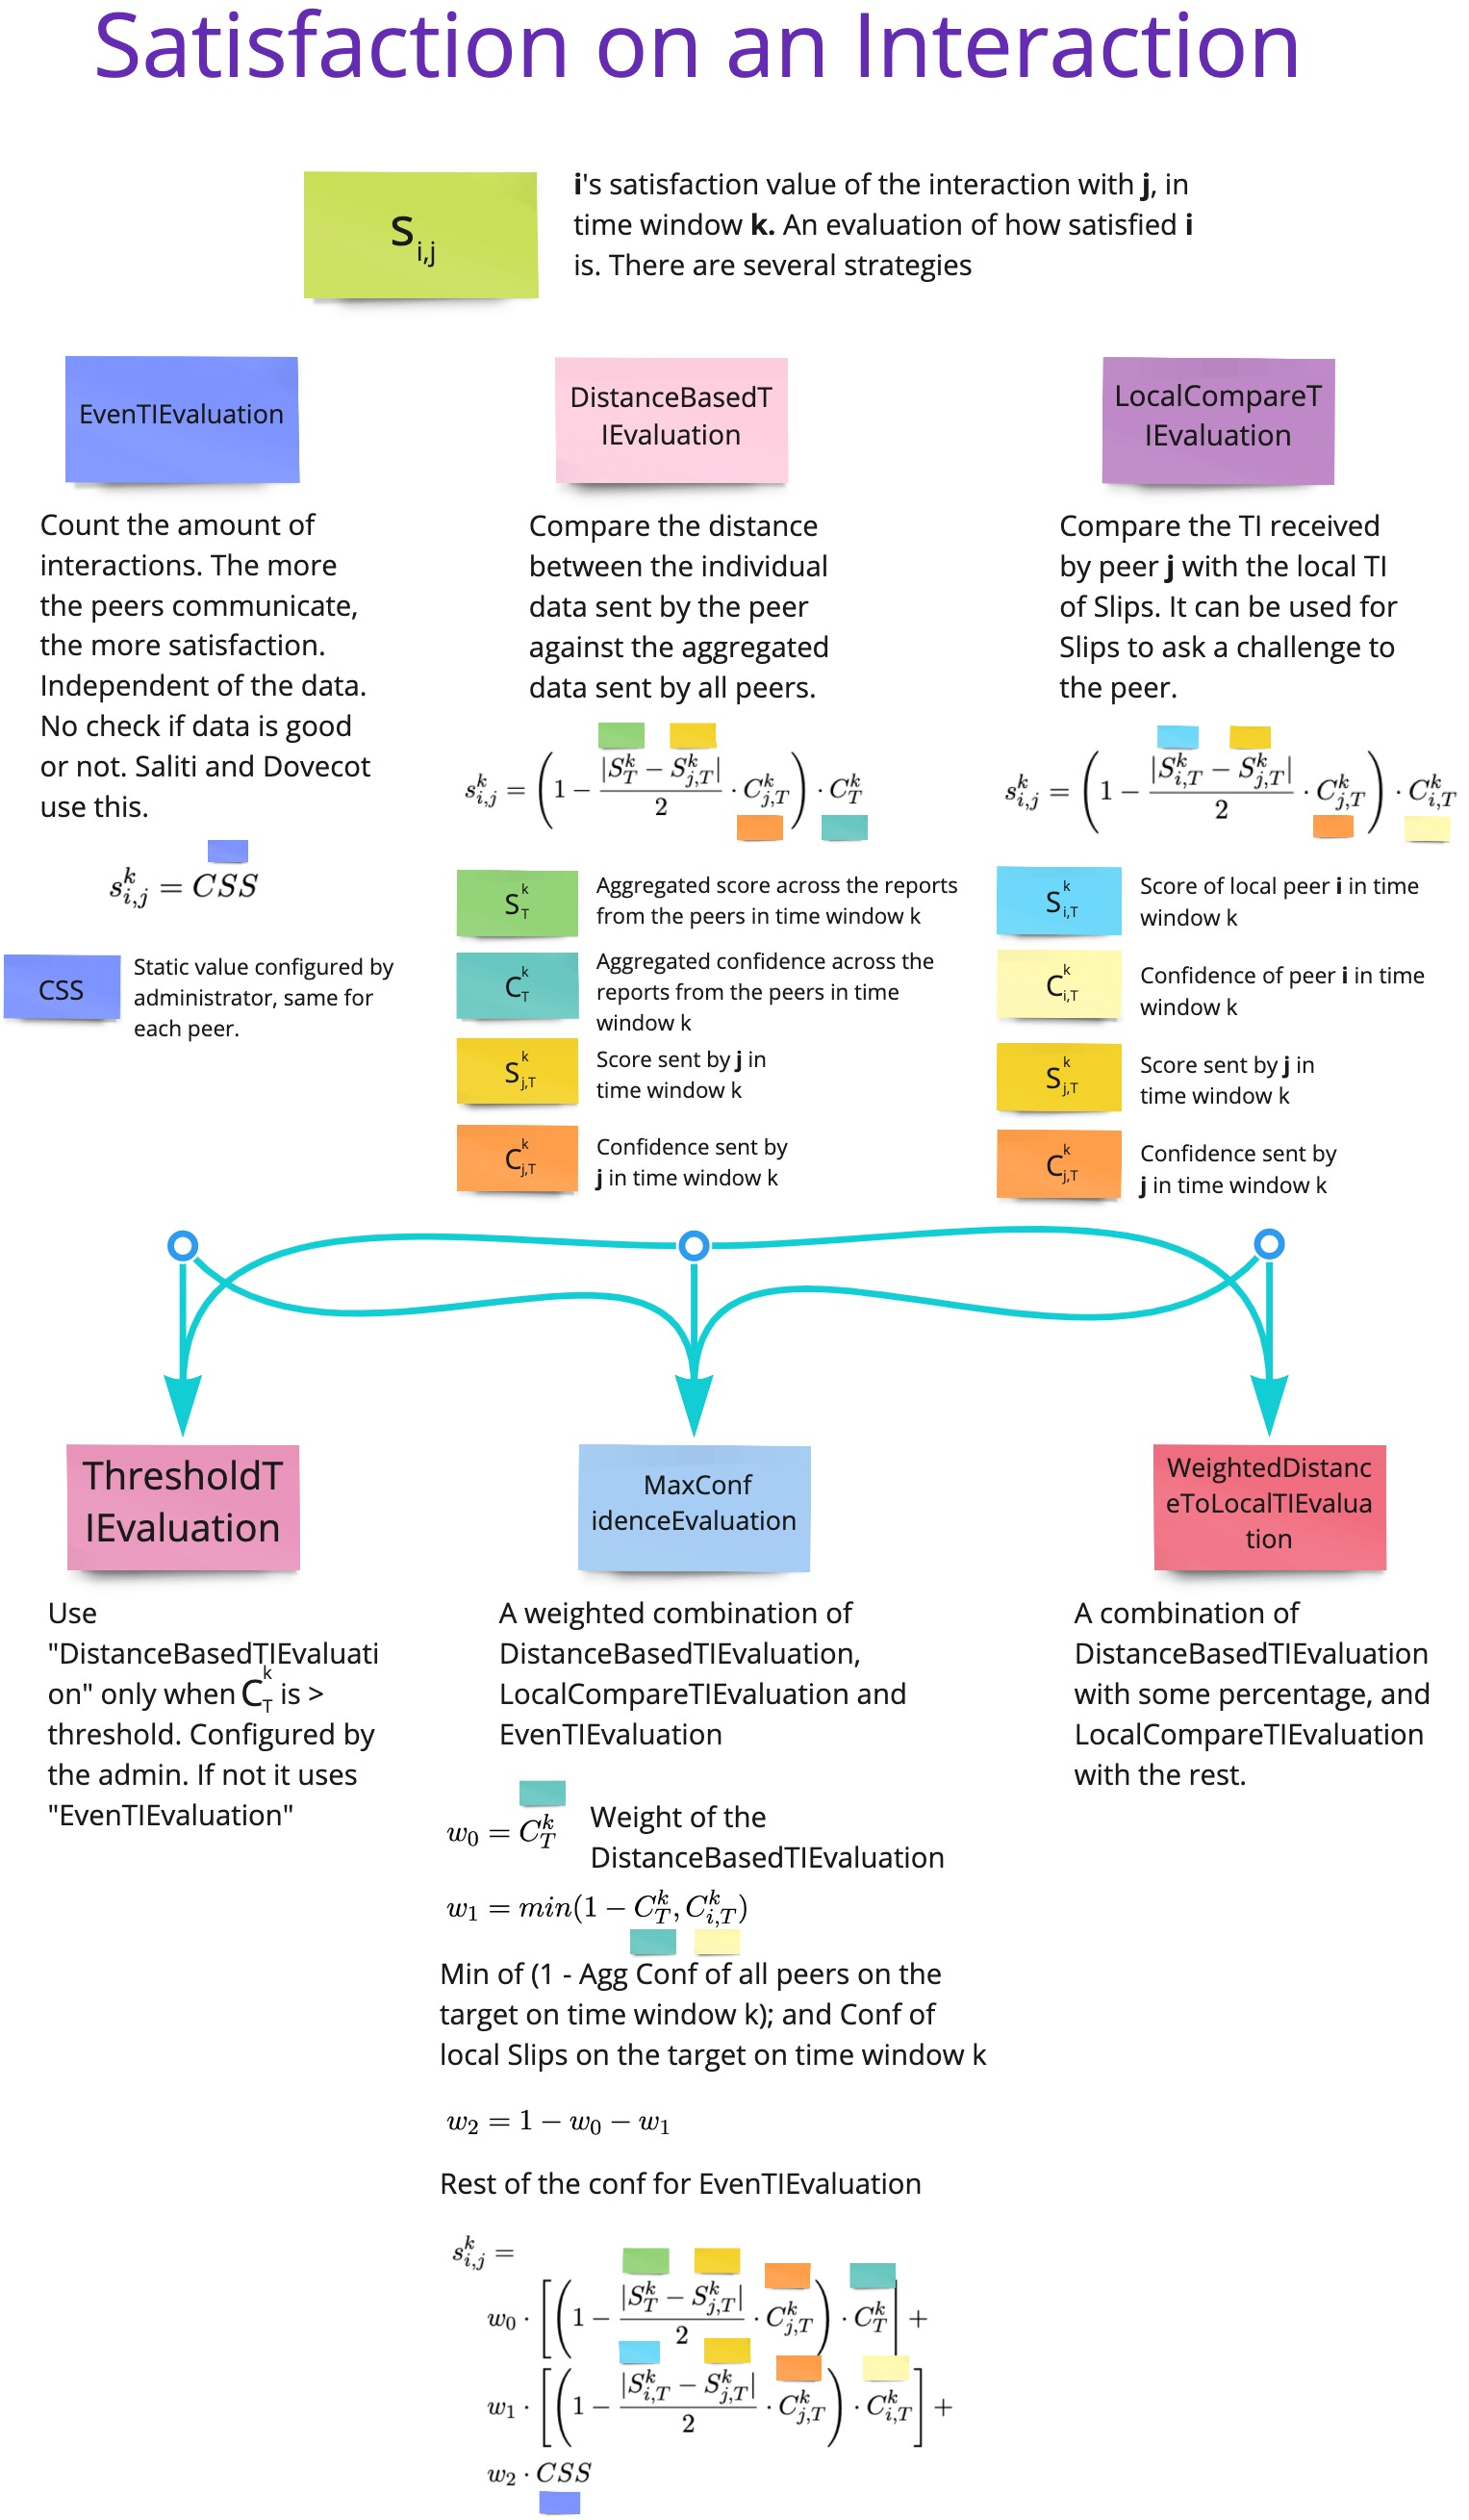
\includegraphics[height=0.95\textheight]{assets/interaction_evaluation.jpeg}
    \caption{Overview of interaction evaluation methods}
    \label{fig:overview-of-interaction-evaluation-methods}
\end{figure}